\documentclass[11pt]{article}
\usepackage{fullpage}
\usepackage{graphicx}
\usepackage{float}
\usepackage{amsmath}
\usepackage{url}

% for citations
\usepackage{hyperref} % Load hyperref before biblatex
\usepackage[natbib, maxcitenames=3, style=apa]{biblatex}
\addbibresource{references.bib}

\title{CS63 Spring 2024\\ Local Spatial Relations in Time-Series EEG Data}
\author{Abdelrahman Abdelmonsef, Mehtap Yercel}
\date{\today}

\begin{document}

\maketitle

\section{Introduction}

% Your paper should be 4-6 pages long.  In this section you should give a broad introduction to your project. Assume that you are writing to an audience that is familiar with AI, but may not know the details of the particular technique that you are using.  You should give an overview of the approach being explored, and how you applied it to a particular problem. 

Convolutional Neural Networks (CNNs) are neural networks that use convolutional layers to extract and recognize common features in the input data. These networks are known to perform well on data exhibiting spatial locality relations, such as images, where the filters applied in the convolutional layers extract patterns from these relations \parencite{meedencnn, mitchellcnn}. 

Our project aims to investigate whether time-series data, denoting chronological data recorded over a time span \parencite{timeseriesdata}, exhibits spatial locality similar to images. Specifically, we aim to explore the spatial locality of electroencephalogram (EEG) signals. EEG measures brainwave activity via electrodes located on the participant's scalp, offering insights into brain function during specific tasks or conditions.

We will be using the EEGEyeNet dataset \parencite{eegeyenet}, which is a dataset containing EEG recordings from 356 adults between the ages of 18-80 that were asked to perform multiple eye-tracking tasks. For the purposes of our project, we will only be using data from the left/right antisaccade task. During this task, participants were instructed to look the opposite direction from a cue of either left or right that was displayed on a screen in front of them. The EEG net used in this task had 129 electrodes placed in a circular pattern around the participant's head, as shown in Figure \ref{eeg_net}, with each electrode recording EEG signals for a duration of the participants' performing the task (500 milli-seconds). 

Our objective is to assess whether local spatial relationships persist within the relative positioning of electrodes around the participant's head and within the chronological sequence of EEG data. To this end, we'll create two additional versions of the dataset: electrode-shuffled and time-shuffled. The electrode-shuffled dataset involves rearranging data along the electrode axis, simulating a physical alteration in electrode placement within the EEG net. The time-shuffled dataset corresponds to shuffling the chronological ordering of data within EEG recordings, potentially distorting the representation of normal brain function.

By evaluating CNN performance across these datasets, we aim to validate or refute the presence of local spatial relations within time-series EEG data. A decline in the performance on shuffled datasets compared to the original dataset would imply the existence of disrupted spatial relations in the original data.

\begin{figure}[H]
\begin{center}
\fbox{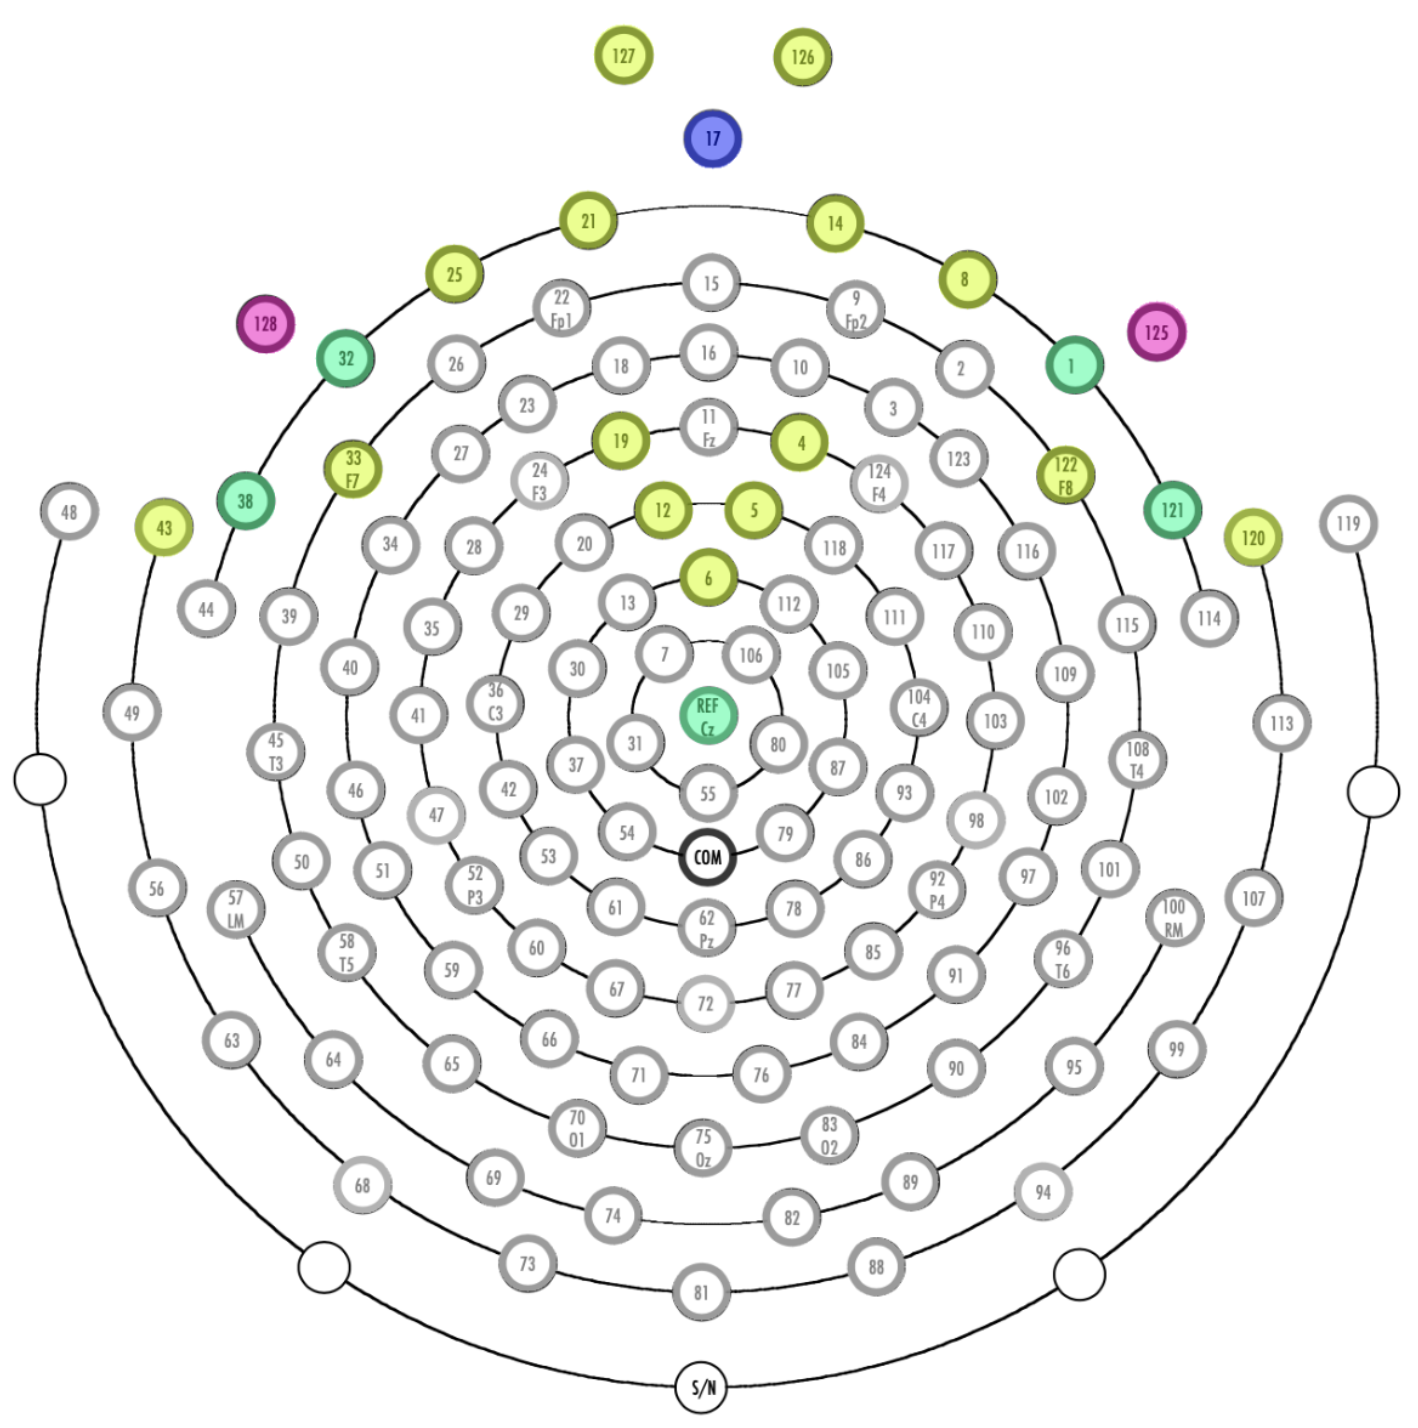
\includegraphics[scale=0.35]{eeg_net.png}}
\end{center}
\caption{Layout of 129 electrodes on the EEG net \parencite{electrode}.}
\label{eeg_net}
\end{figure}

\section{Methods}

% In this section you should explain the details about your project.

% For example, if your project is based on a Kaggle competition, this should include describing the data set used (number of patterns, number of features, description of features, any preprocessing that was necessary) and its source.

% You should provide all of the parameter settings used (such as learning rate, etc.). You should also provide details about how the system was trained, and how you determined when to end training.

% Details about how to test and run your \emph{code} should NOT be given in the paper, but should instead be described in the README file in the lab directory. 

% SECTIONS
% 1. Downloading the model and cleaning it up 
% 2. Data precprocessing
% 3. Running the model
% 4. Statistical analysis

In this section, we will detail the steps we took to select a CNN and prepare data for model training and evaluation.

\subsection{Data Description}

The EEGEyeNet dataset comprises 30,825 pre-processed EEG recordings, each containing 500 * 129 values. Each value corresponds to an EEG signal recorded from one of the 129 electrodes across 500 time points. The label for each recording is binary, denoted as 0 or 1, indicating whether the subject was looking left or right during the recording.

The EEGEyeNet GitHub repository \parencite{code} provides detailed information on the data acquisition and pre-processing procedures. To prepare the dataset for our experiments, we executed the following processing steps:

\begin{enumerate}
    \item Due to the dataset's substantial size (15GB), we truncated it to utilize only the first 10,000 records in our experiments. This reduction ensured compatibility with TensorFlow's computational and memory constraints in our experimentation environment.
    
    \item Subsequently, we generated two additional versions of the truncated dataset: one with data shuffled along the electrode axis and another with data shuffled along the time axis.

    To create the electrode-shuffled version, we randomly permuted the numbers from 0 to 128 (inclusive). Then, for each record in the dataset, we reordered the 129 electrode readings based on this permutation while preserving the time-ordering of the data per electrode, thereby shuffling the electrodes' relative positions.

    To generate the time-shuffled version, we generated a random permutation of the numbers from 0 to 499 (inclusive). For each record in the dataset, we reordered the 500 data points per electrode based on this permutation, thus maintaining the relative positions of electrodes while shuffling the time ordering per electrode.

    \item For each of the three datasets described above, we partitioned the data into training, validation, and testing sets using a 70-15-15 split.
    
\end{enumerate}


\subsection{Model Description}

For experimentation, we used a standard one-dimensional CNN, based upon the CNN used in \cite{eegeyenet}. The original CNN contains 12 modules with an additive shortcut layer following each three modules. This is later followed by global average one-dimensional pooling and a final dense layer with an output shape of 1 and a sigmoid activation function. Each module has (1D-)convolution, batch normalization, ReLU activation, and max pooling. For convolutions, 16 filters of size 64 were used, and for the pooling, a kernel of size 2 and stride of 1 were used. Each shortcut layer performs a convolution followed by batch normalization.

Upon applying the original CNN on the truncated dataset, it very quickly led to over-fitting. As a result, we adjusted the number of modules in the CNN to only 4 with only one shortcut layer, keeping everything else the same. Although training using this reduced-size model still results in over-fitting, the model's generalization capability improved compared to the bigger model. Also, the model showed over-fitting effects later, relative to the original CNN.

\subsection{Training Procedures}

We conducted training and testing of the CNN on three distinct versions of the time-series dataset: the original dataset and the two shuffled versions. Accuracy served as the metric to gauge the model's performance. Here, accuracy denotes the proportion of correctly classified labels (left/right) by the model when applied to EEG signal samples in the testing split.

The training-testing procedure was iterated five times for each dataset condition, yielding a total of 15 scores. Table \ref{parameters} outlines the parameter configurations employed across all experiments. Subsequently, the accuracies obtained from the 15 runs were aggregated to calculate the mean per dataset and used for further statistical analysis.

\begin{table}[H]
\begin{center}
\begin{tabular}{|l|r|} \hline
{\bf Parameters} & {\bf Settings} \\ \hline
Learning rate & 1e-4 \\
Batch Size & 64 \\
Kernel Size & 64 \\
Num Filters & 16 \\
Epochs & 30 \\ 
Loss Function & Binary Cross-Entropy Loss (bce) \\ \hline
\end{tabular}
\caption{Model parameters for training.}
\label{parameters}
\end{center}
\end{table}

\subsection{Statistical Analysis}

The purpose of the statistical analysis procedures is to investigate whether the variations in scores across the experiments within each dataset hold statistical significance. To achieve this, we employed an Analysis of Variance (ANOVA) test, a widely recognized statistical tool for discerning significant differences among group means.

First, we ran the data through the Shapiro-Wilk test for assessing normality and Levene's test for evaluating the homogeneity of variances. Passing both tests validated the suitability of employing ANOVA to gauge statistical significance. We then conducted the ANOVA test, where a significance level of 0.05 was adopted as the threshold for determining statistical significance.

\section{Results \& Discussion}

% In this section you should show and analyze the results. Measure the performance of your system, and if possible compare your performance to other implementations. Use tables and figures to illustrate the results. You should also discuss what sorts of conclusions can be drawn from these results; what did you learn, what are the important takeaways for a reader, etc.

% Even if your project is not as successful as you'd hoped, you still need to show and discuss results. This section is one of the key parts of any scientific paper. Be sure to provide adequate information so that the reader can evaluate the outcomes of your experiments. 

Table \ref{runs} shows the obtained testing accuracies for 5 runs of training and testing the CNN model on each of the 3 datasets, along with the average performance for each.

\begin{table}[H]
\begin{center}
\begin{tabular}{|l|c|c|c|} \hline
{\bf Runs} & {\bf Original} & {\bf Electrode Shuffled} & {\bf Time Shuffled} \\ \hline
Run 1 & 70.63 & 62.90 & 54.56\\
Run 2 & 71.03 & 67.99 & 51.52\\
Run 3 & 68.45 & 66.34 & 54.03\\
Run 4 & 72.02 & 62.50 & 55.09\\
Run 5 & 70.30 & 68.19 & 55.36\\
\textbf{Average Testing Accuracy (\%)} & \textbf{70.49} & \textbf{65.58} & \textbf{54.11}\\ \hline
\end{tabular}
\caption{Testing accuracy of the CNN model over 5 runs on three different dataset conditions.}
\label{runs}
\end{center}
\end{table}

As shown, on average, the CNN model performed the best on the original dataset as compared to the electrode-shuffled and time-shuffled versions. A one-way ANOVA test was applied twice: one comparing the original scores to the electrode-shuffled and another comparing the original scores to the time-shuffled. The p-values obtained were $p < 0.01$ and $p < 0.0001$, respectively. Furthermore, a one-way ANOVA was used to observe that the difference between the performances of the two shuffled datasets is statistically significant with a p-value of $p < 0.0001$. Using a significance level of 0.05, we can say that both differences are statistically significant.

These results suggest that the dip in performance experienced when the ordering of the data was shuffled across both the electrode and time dimensions can't be attributed to random chance. Rather, these differences can be attributed to the disruptions of the patterns arising from the local spatial relations within the original ordering of the data. Electrode-shuffling the data equates to shuffling the locations of the electrodes on the EEG net. Given that the CNN performed worse on the electrode-shuffled data, this might indicate that there are spatial patterns that arise from the locations of the electrodes around the participant's head that are disrupted when the electrodes are shuffled, which may cause the CNN to perform worse. Similarly, time-shuffling the data shuffles around the datapoints within each EEG, which essentially creates a new  EEG that may be unrepresentative of actual brain functions. Given that the CNN performed worse on the time-shuffled data, this may indicate that there are important patterns within an authentic EEG recording that are disrupted when the time data is shuffled, which would explain the CNN's even worse performance on this dataset compared to electrode-shuffled.

\section{Conclusions}

% This section should sum up what you did and what you found. It is also ppropriate to mention things you would have liked to do but didn't have time for as `future work.'

In this project, we were interested in examining whether time-series EEG data exhibits local spatial relations that are present in the relative-ordering of the electrodes and chronological EEG recordings per electrode. 

To do so, we trained a CNN model on three different versions of the same EEG dataset to examine whether disrupting the ordering of the data would disrupt local spatial relations, as indicated by the CNN's worsening performance. Our CNN model performed better on the original time-series data with the local spatial relations intact compared to the electrode-shuffled and time-shuffled datasets. This supports the idea that there may be local spatial relations in the time-series dataset that allows the CNN to perform well on the left/right antisaccade classification task. In addition, our CNN model also performed better on the electrode-shuffled dataset as opposed to the time-shuffled dataset, which indicates that shuffling the chronological time-series data disrupts local spatial relations more than shuffling electrodes do.

We were only able to perform 5 runs per dataset condition; however, further repetitions of training the CNN should be done to confirm the findings of this project. Furthermore, in our initial planning of this project, we were also interested in comparing the performance of a feed-forward neural network to the CNN. While we had to forego this idea due to computational constraints, it would be interesting to compare the performance of our CNN on the EEG dataset to that of a feed-forward neural network to see if the ability of the CNN to recognize features based on local spatial relations would allow it to perform better.

\section{Acknowledgements}

% You should clearly acknowledge any outside sources of help you had. In particular, if you used resources from the internet, you should describe what they were and how they were used.  Note that this applies to all phases of the project, including coding, analysis, and writing. This doesn't need to be long, but should include enough detail it's clear what you did yourself and what you got from elsewhere.

% For instance, you might say that you got help brainstorming and finding good libraries to use from Professor A, then got help figuring out how to apply statistical tests from Professor B, and finally used ChatGPT to generate an outline for the `Introduction' section.

We want to thank Professor Lisa Meeden and Professor Ben Mitchell for their support and guidance throughout this project. Professor Meeden helped us brainstorm our current project idea when our initial plan did not go accordingly. We also would like to thank Ard Kastrati, a co-author of the EEGEyeNet paper, for allowing us to use their code and datasets in this project. Mr. Kastriti was essential to the success of this project as they answered the questions we had regarding their datasets and code. Lastly, we used SciPy for statistical analysis and ChatGPT to generate Latex code for properly formatting the references.bib file and the references page and fix grammatical errors in the original draft of the paper.

\pagebreak
\printbibliography

\end{document}